\documentclass[11pt]{article}
\usepackage[latin2]{inputenc}
\usepackage{a4wide}
\usepackage{graphicx}
\usepackage{hyperref}
\hypersetup{colorlinks=true,linkcolor=blue}
\title{Flexy Beast Documentation}
\author{ThingDoc}

\begin{document}

\maketitle
\begin{center}

\includegraphics[width=8cm]{logo.png}
\end{center}
The Flexy Beast is a wrist-powered prosthetic hand for the e-NABLE Project. This is a mashup of the Parametric Cyborg Beast by MakerBlock and the Flexy Hand by Steve Wood/Gyrobot. Like the Flexy-Hand, the Flexy Beast uses flexible joints to replace the Chicago screws and elastics used on previous e-NABLE designs. This makes the hand lightweight, less expensive, better looking, more adaptable for smaller sizes, and easier to assemble and use.

\newpage

\tableofcontents

\newpage

\section{Bill of Materials}
List of things you need to build the machine divided by categories.

\subsection{Prerequisites!}
\begin{itemize}
\item 1x \hyperlink{thing_config\_file}{Configuration File}
\end{itemize}

\subsection{Flexible}
\begin{itemize}
\item 10x \hyperlink{thing_flexy\_joint}{Flexy Joint}
\end{itemize}

\subsection{Other}
\begin{itemize}
\item 5x \hyperlink{thing_string}{String}
\end{itemize}

\subsection{Printed}
\begin{itemize}
\item 4x \hyperlink{thing_finger\_tip}{Finger Tip}
\item 5x \hyperlink{thing_finger\_tip\_mold}{Finger Tip Mold}
\item 1x \hyperlink{thing_palm}{Palm}
\item 5x \hyperlink{thing_finger\_base}{Finger Base}
\item 1x \hyperlink{thing_thumb\_tip}{Thumb Tip}
\end{itemize}

\newpage

\section{Things Overview}
List of things and their descriptions.

\hypertarget{thing_thumb\_tip\_grip}{\subsection{Grippy Thumb Tip}}
Molded silicone grippy thumb tip

\hypertarget{thing_config\_file}{\subsection{Configuration File}}
Configuration settings for Flexy Beast, required to generate correctly sized STLs of the printed parts. See the Configuration File Assembly instructions to set this up.

\hypertarget{thing_string}{\subsection{String}}
Just some string

\hypertarget{thing_finger\_tip\_grip}{\subsection{Grippy Finger Tip}}
The Flexy Beast fingers can be made with silicone finger pads for improved grip. These finger pads are designed to be easily removeable and replaceable by hand, but attach firmly enough to stay on during use. Dragon Skin 10 silicone produces very soft and grippy pads; Dragon Skin 30 is tougher.
\includegraphics[width=4cm]{images/finger\_tip\_grip.jpg}

\hypertarget{thing_finger\_tip}{\subsection{Finger Tip}}
Distal phalanx of fingers - rendered from parts/finger_tip.scad
\includegraphics[width=4cm]{images/finger\_tip.png}

\hypertarget{thing_finger\_base}{\subsection{Finger Base}}
Proximal phalanx for all digits (fingers and thumb) - rendered from parts/finger_base.scad
\includegraphics[width=4cm]{images/finger\_base.png}

\hypertarget{thing_thumb\_tip}{\subsection{Thumb Tip}}
Distal phalanx of thumb - rendered from parts/thumb_tip.scad
\includegraphics[width=4cm]{images/thumb\_tip.png}

\hypertarget{thing_thumb\_assembly}{\subsection{Assembled Thumb}}

\hypertarget{thing_palm}{\subsection{Palm}}
Palm - rendered from parts/palm.scad
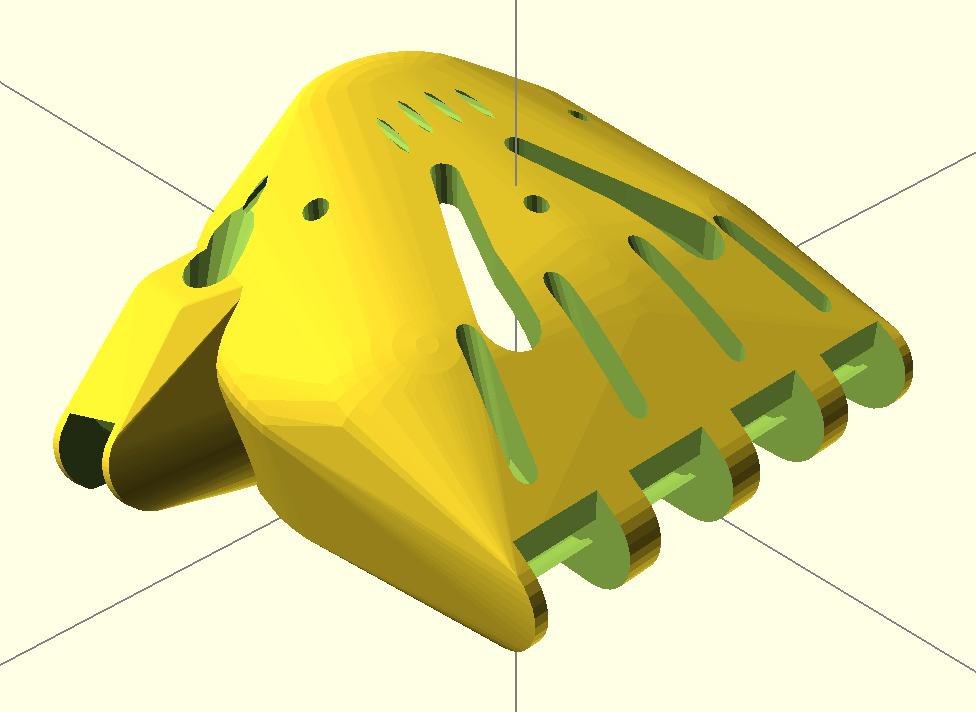
\includegraphics[width=4cm]{images/palm.png}

\hypertarget{thing_flexy\_joint}{\subsection{Flexy Joint}}
Flex joint - can be molded in silicone or printed in Filaflex. The Configuration File instructions will help you find a good size for these.

\hypertarget{thing_finger\_assembly}{\subsection{Assembled Finger}}

\hypertarget{thing_finger\_tip\_mold}{\subsection{Finger Tip Mold}}
Mold for casting silicone finger tip grip - rendered from parts/finger_tip_mold.scad
\includegraphics[width=4cm]{images/finger\_tip\_mold.png}

\newpage

\section{Assembly Instructions}

\subsection{Assemble Configuration File}Steps:
\begin{enumerate}
\item Open config.scad in your favorite text editor.
\item As per the normal Cyborg Beast instructions, measure the width of the knuckles in the non-affected hand and convert to millimeters.
\item Add 5 to that result and then divide by 55.
\item Replace the x-, y-, and zScaleFactor variables in config.scad with that number.
\item If desired, adjust the proportions of the hand by changing those variables individually. xScaleFactor controls the width of the hand, yScaleFactor controls the length, and zScaleFactor controls the height.
\item Open assembly.scad in OpenSCAD to check that the flexy joint holes are not too large for the hand (should only be necessary for small children). If necessary, reduce the jointDia and jointThick variables. jointDia=5 and jointThick=2 is a good amount for smaller hands.
\item Set the fingerPads variable to true or false depending on whether you want to cast silicone finger pads for improved grip.
\item Open palm.scad, finger\_base.scad, finger\_tip.scad, and thumb\_tip.scad in OpenSCAD, render each part (F6), and export as STL, then print. Suggested print settings are 0.2mm or smaller layer height, 3 perimeters, and 25\% rectilinear or hexagonal infill.
\end{enumerate}

\subsection{Assemble Grippy Finger Tip}
Things needed:
\begin{itemize}
\item 1x \hyperlink{thing_finger\_tip}{Finger Tip}
\item 1x \hyperlink{thing_finger\_tip\_mold}{Finger Tip Mold}
\end{itemize}
Steps:
\begin{enumerate}
\item Print the finger tip and mold.\\ 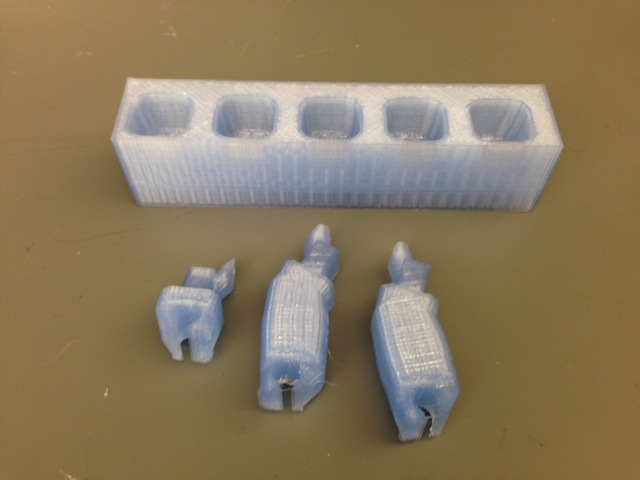
\includegraphics[width=4cm]{images/pad\_casting/Printed parts.jpg}
\item Insert the string through the fingertip and tie off the end prior to molding (not shown in all photos here).\\ \includegraphics[width=4cm]{images/pad\_casting/Fingertip with string.jpg}
\item Mix silicone according to the instructions from the supplier. Wear gloves and follow the supplier's safety instructions while working with liquid silicone.\\ 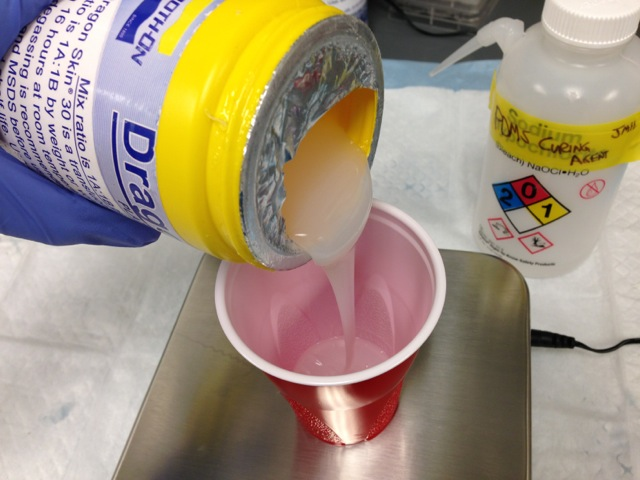
\includegraphics[width=4cm]{images/pad\_casting/Pouring part A.jpg}
\item Pour the liquid silicone to mostly fill the fingertip mold.\\ 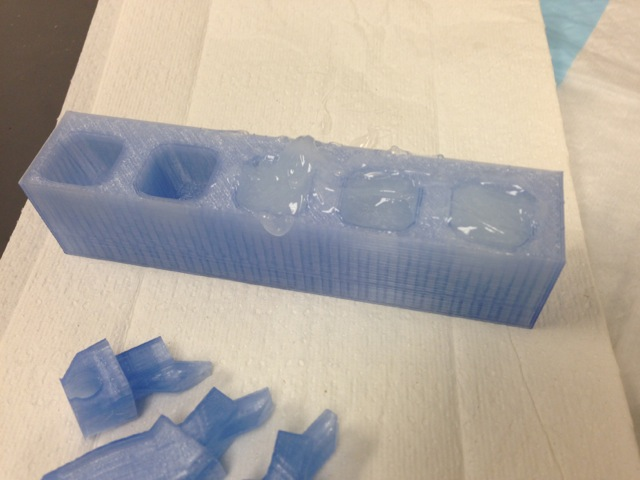
\includegraphics[width=4cm]{images/pad\_casting/Poured into mold.jpg}
\item Insert the printed fingertip piece into the filled mold.\\ 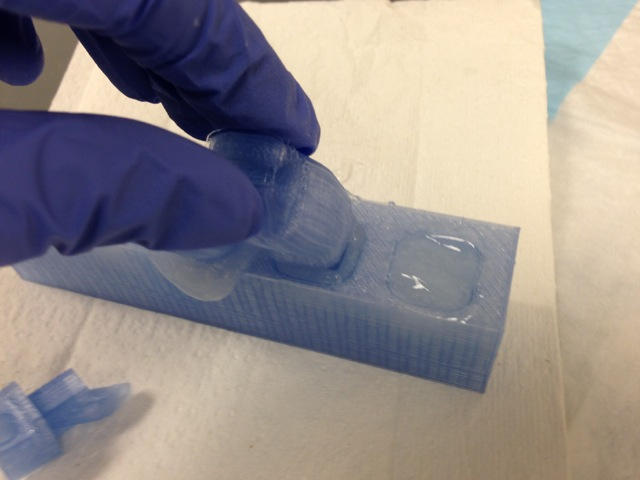
\includegraphics[width=4cm]{images/pad\_casting/Inserting phalange.jpg}
\item Remove any excess silicone. If necessary, use tape to hold the phalange in place.\\ 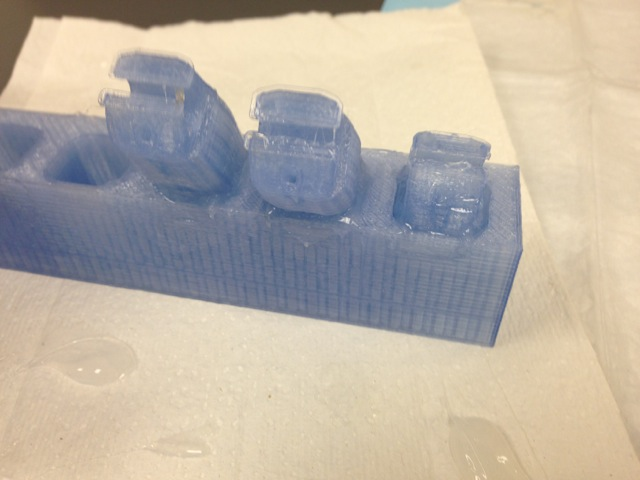
\includegraphics[width=4cm]{images/pad\_casting/Phalanges in mold.jpg}
\item When the silicone is cured, remove the fingertip and silicone pad from the mold. The pad may stay on the fingertip or it may need to be removed separately.\\ 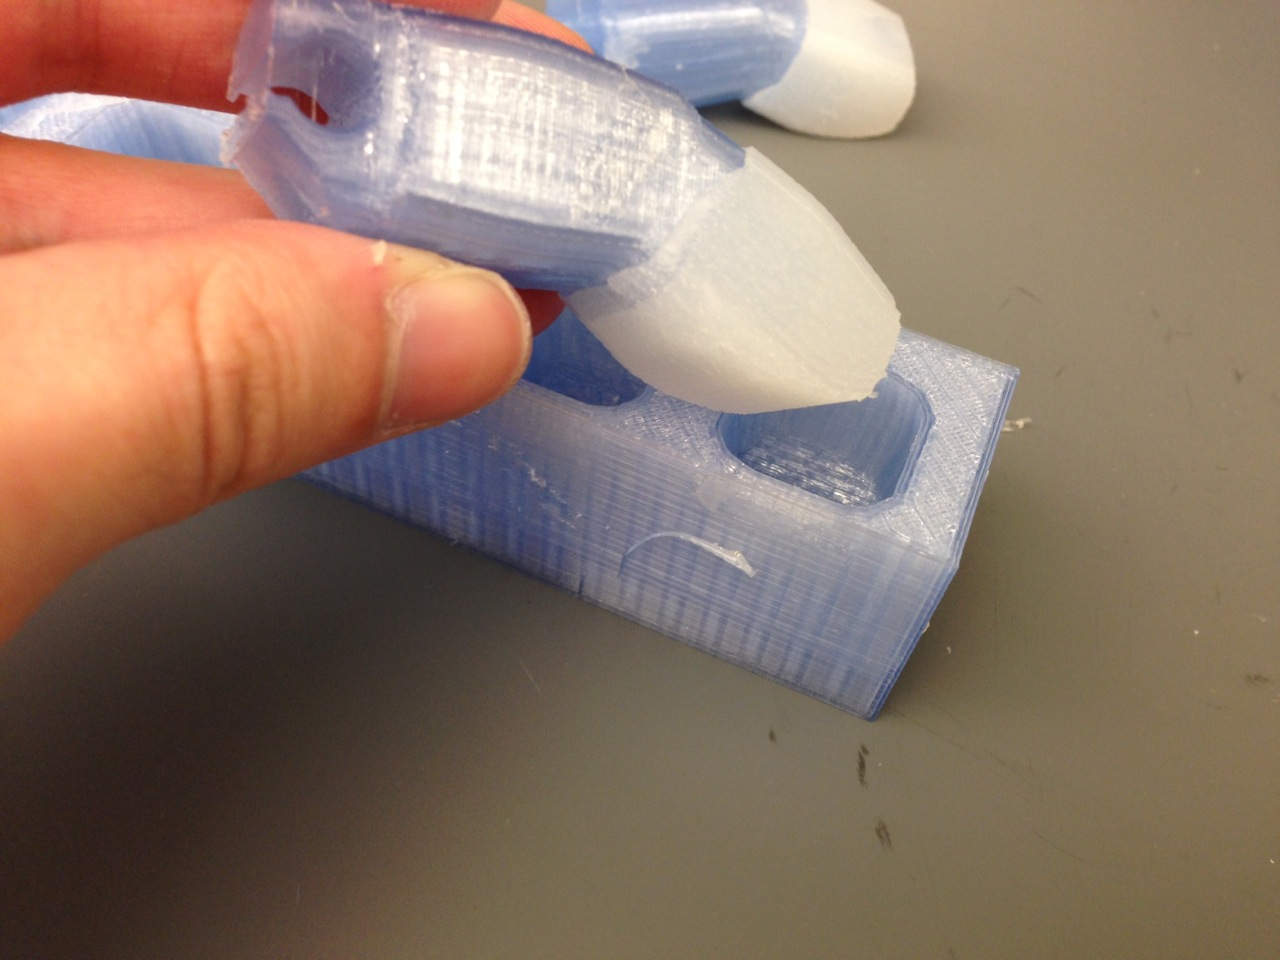
\includegraphics[width=4cm]{images/pad\_casting/Removing from mold.jpg}
\item If the pad came off the fingertip during demolding, it can be reattached by pushing it over the end of the fingertip.\\ 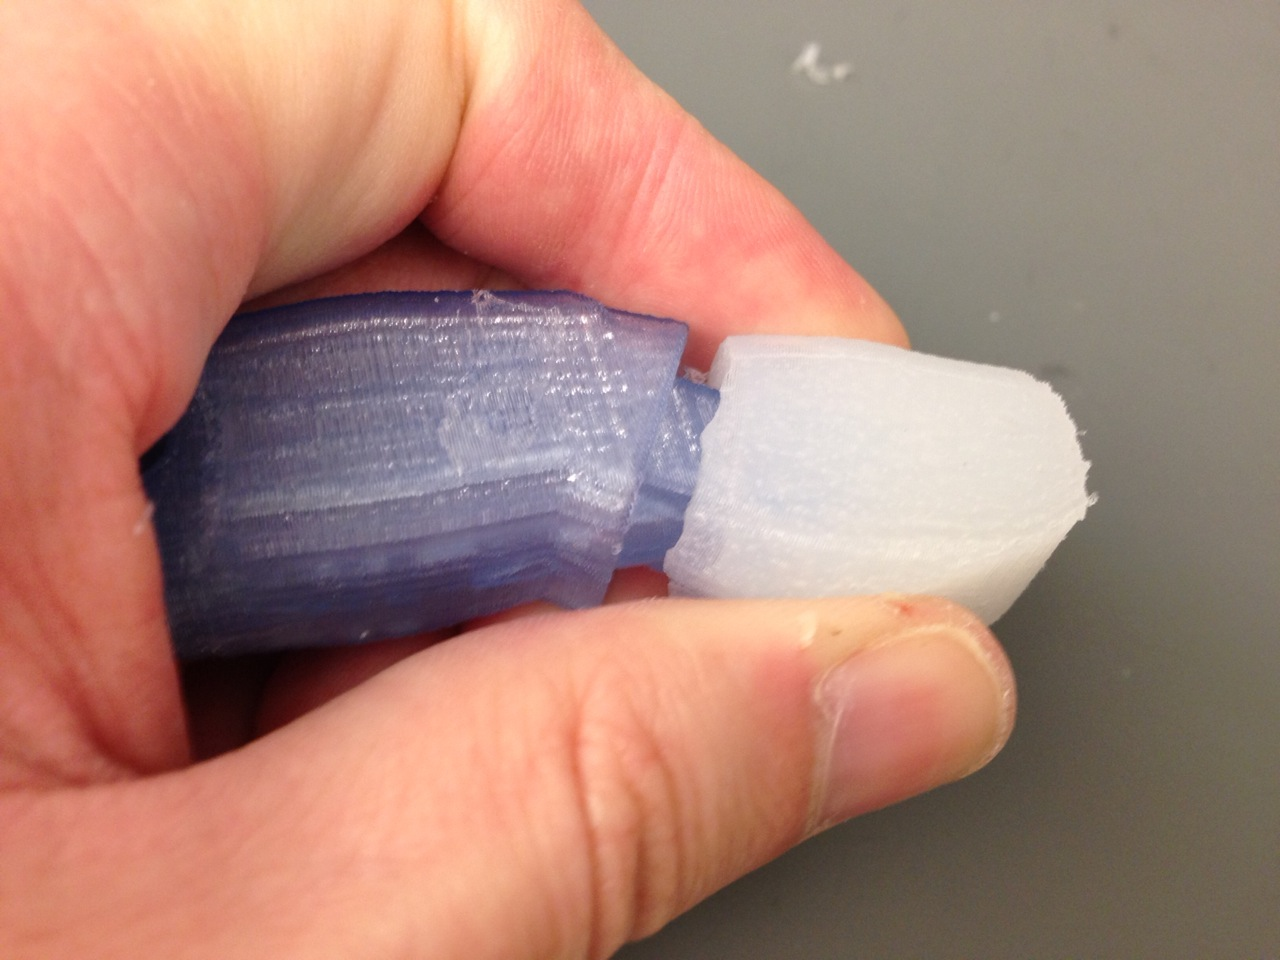
\includegraphics[width=4cm]{images/pad\_casting/Installing finger pad.jpg}
\item If necessary, use an x-acto knife to trim off excess silicone so that the edges of the pad are flush with the edges of the fingertip.
\item The fingertip pads are finished. Continue installing them onto the hand.\\ 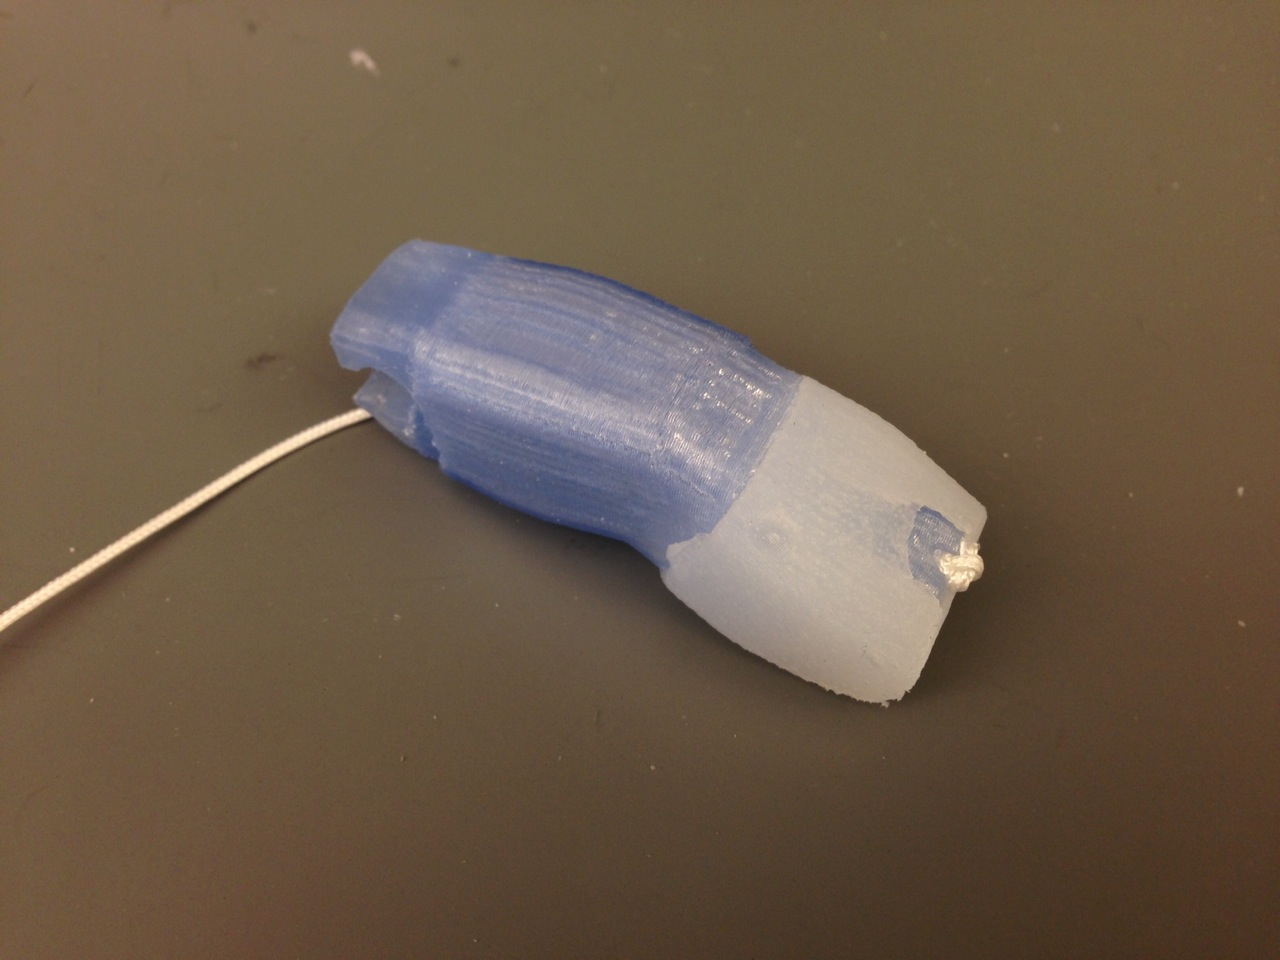
\includegraphics[width=4cm]{images/pad\_casting/Assembled fingertip.jpg}
\end{enumerate}

\subsection{Assemble Flexy Beast}
Things needed:
\begin{itemize}
\item 1x \hyperlink{thing_palm}{Palm}
\item 1x \hyperlink{thing_thumb\_assembly}{Assembled Thumb}
\item 1x \hyperlink{thing_config\_file}{Configuration File}
\item 4x \hyperlink{thing_finger\_assembly}{Assembled Finger}
\end{itemize}
Steps:
\begin{enumerate}
\item Print the palm, thumb base, thumb tip, and four each of the finger base and tip. These can be scaled as needed in each dimension using the x-, y-, and zScaleFactor variables in the OpenSCAD code.
\item Insert a string through each fingertip (the hole may need to be drilled slightly to deburr) and tie it off on the end.\\ \includegraphics[width=4cm]{images/hand\_assembly/Fingertip with string.jpg}
\item After making the 3D printed parts and flexible joints, slide a flex joint into the proximal end of each finger.\\ 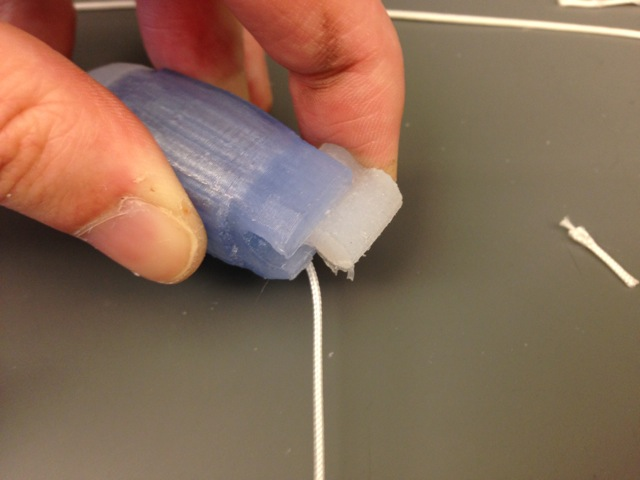
\includegraphics[width=4cm]{images/hand\_assembly/Inserting joint.jpg}
\item Use a flat screwdriver or other thin, flat tool to insert the other end of the joint into the corresponding slot on the next inner segment.\\ 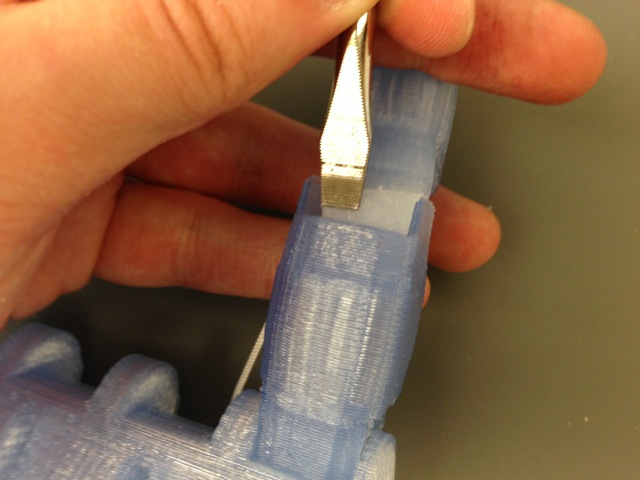
\includegraphics[width=4cm]{images/hand\_assembly/Inserting joint with screwdriver.jpg}
\item Route the string through all the finger segments.\\ 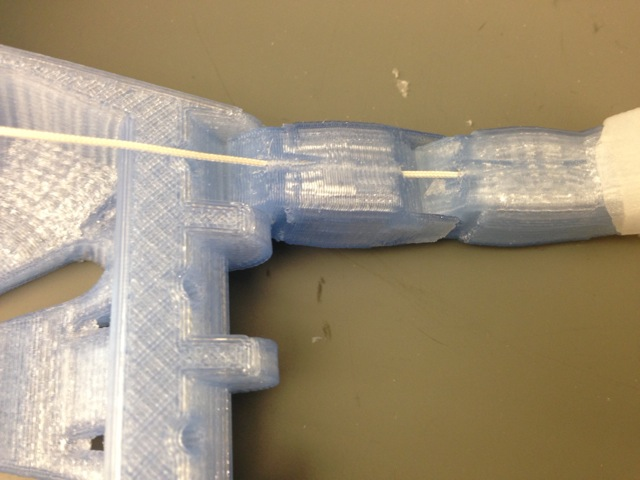
\includegraphics[width=4cm]{images/hand\_assembly/String routing.jpg}
\item Route the string through the palm.\\ 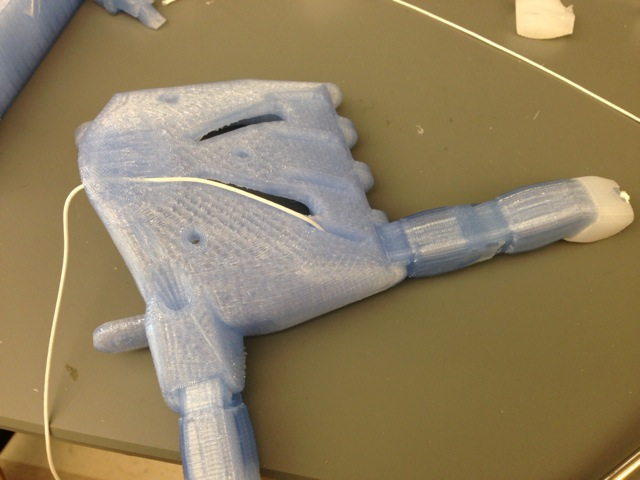
\includegraphics[width=4cm]{images/hand\_assembly/String routing through palm.jpg}
\end{enumerate}

\newpage

\end{document}